Our plan for the project relies primarily on previous experiences earlier in our studies. The development of the system will be carried out using AGILE development or modified SCRUM. A development team of two won't benefit from a full SCRUM approach, and it is not appropriate for this type of project. However, we think certain aspects of SCRUM, such as sprints and milestones can be useful to a team of any size. \\ \\We will use the V-model for test specification, and the ASE model for the project flow. The V-model is a way of breaking down complex systems into smaller ones, and then testing it from the ground up. This will result in unit tests of the smallest modules, integration tests where several modules are tested together, and finally a system test incorporating all modules of the system. 


\begin{figure}[H]
	\centering
	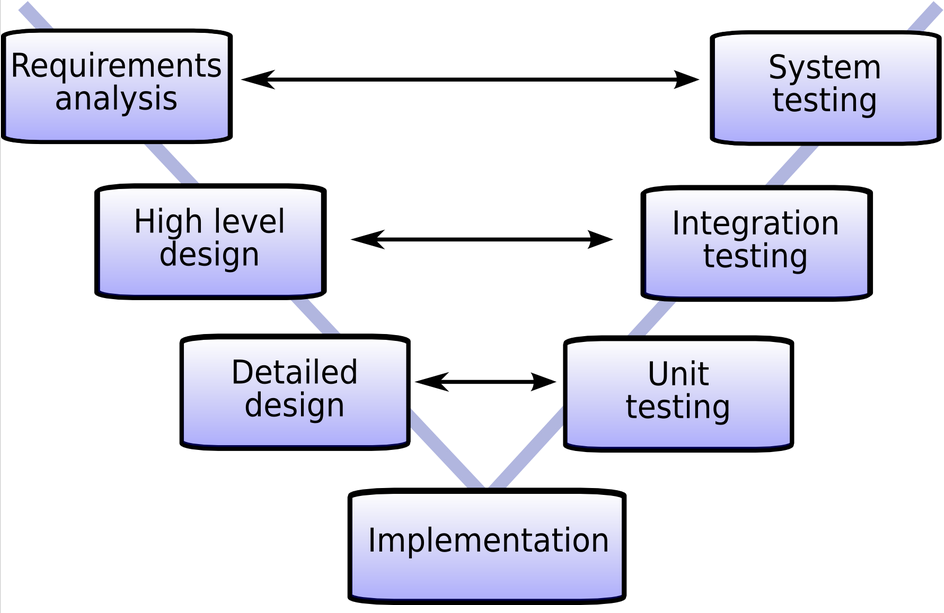
\includegraphics[max width=1\linewidth]{Billeder/V-model.png}
	\caption{V model\cite{V-model}}
	\label{fig:V model}
\end{figure}


The ASE model details a development plan for a project. First, the overall goal for the project is described followed by a requirements specification. Then, the system architecture is divided into hardware and software sections so these can be detailed and developed individually. Finally, the hardware and software architectures are tested in an integration test, and the product test can be carried out. This development plan closely resembles the workflow in the V-model, and the two complement each other well.


\begin{figure}[H]
	\centering
	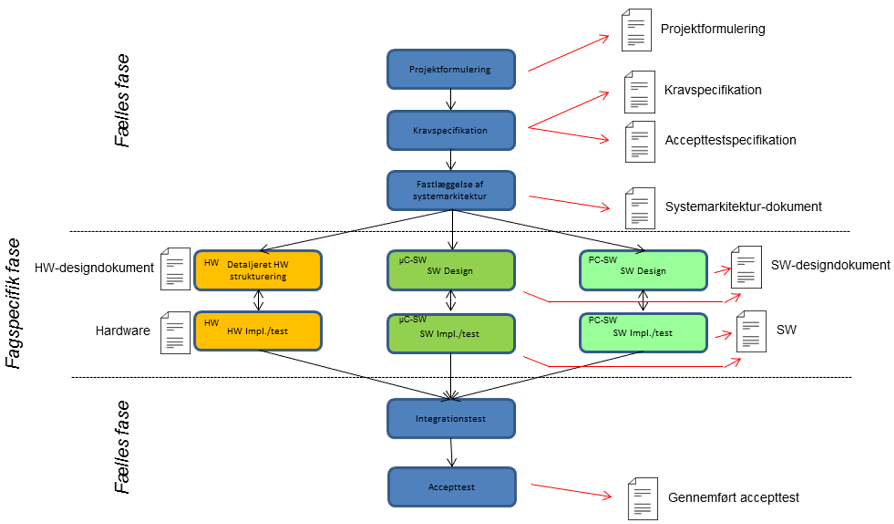
\includegraphics[max width=1\linewidth]{Billeder/ASE-model.png}
	\caption{ASE development model\cite{ASE-model}}
	\label{fig:ASE_model}
\end{figure}


The system will be NMEA compatible, and will use GPS localization. This compatibility is desired since the NMEA specification is used in many different marine tasks, and enables communication between marine electronics such as anemometers, gyrocompasses, echo sounders, sonars, GPS receivers and many other types of instruments used at sea \cite{NMEA}.

It is likely that the system will use a linux core on an Atmel processor, since these are available at EIVA. However, the platform specifics are subject to change.

Finally, a user's guide will be written to aid the end user in using the system.